\chapter{Introducción}
\label{cap:capitulo1}
\setcounter{page}{1}

\begin{flushright}
\begin{minipage}[]{10cm}
\emph{El éxito es la capacidad de ir de fracaso en fracaso sin perder el entusiasmo.}\\
\end{minipage}\\

Winston Churchill\\
\end{flushright}

\vspace{1cm}

La tendencia de la industra hacia la automatización total ha ido en aumento en los últimos años, 
haciendo que la demanda de robots industriales se dispare en todo el mundo. Un ejemplo de ello, son 
las megafactorías en el sector automovilístico. Se tratan de inmensas fábricas con un componente humano
mínimo y con una automatización cada día mayor, mediante el uso de la robótica industrial. \\No solo se hace
uso de grandes robots pesados, sino también de flotas de pequeños pero ágiles robots que desempeñan tareas
en cintas transportadoras, ensamblado de placas base, entre otras.  Debido al aumento en su uso y del progreso 
en estas tecnologías, es necesario formar cada vez más ingenieros que ejercerán en este campo. Es por esto que se 
necesitan herramientas adaptadas a las nuevas tecnologías y fácilmente accesibles para estudiantes y centros.    \\
Por otro lado, la robótica educativa ha nacido como una herramienta innovadora y poderosa en el ámbito de la 
enseñanza. Mediante la integración de robots en las aulas, los estudiantes pueden experimentar el 
aprendizaje de una manera más interactiva y participativa. Desde los centros de educación primaria hasta las 
universidades, la incorporación de la robótica educativa ha experimentado un crecimiento significativo. Esta 
tecnología se adapta de manera excepcional a las necesidades y capacidades de cada etapa educativa.

\section{Robótica industrial}
\label{sec:miseccion} % etiqueta para luego referenciar esta sección

La robótica industrial es la rama de la ingeniería dedicada al diseño, construcción, operación y mantenimiento 
de robots utilizados en la automatización de procesos industriales. Estos robots pueden realizar una amplia variedad 
de tareas, desde la manipulación y transporte de materiales, hasta el ensamblaje y soldadura de piezas. Entre las aplicaciones 
más importantes encontramos las siguientes:

\begin{itemize}
  \item \textit{Automatización de líneas de ensamblaje.} Esta tecnología se encuentra ampliamente asentada en las líneas de  producción 
                                                        del sector automotriz. Un ejemplo son las factorías de Tesla.  
  \begin{figure} [h!]
    \begin{center}
      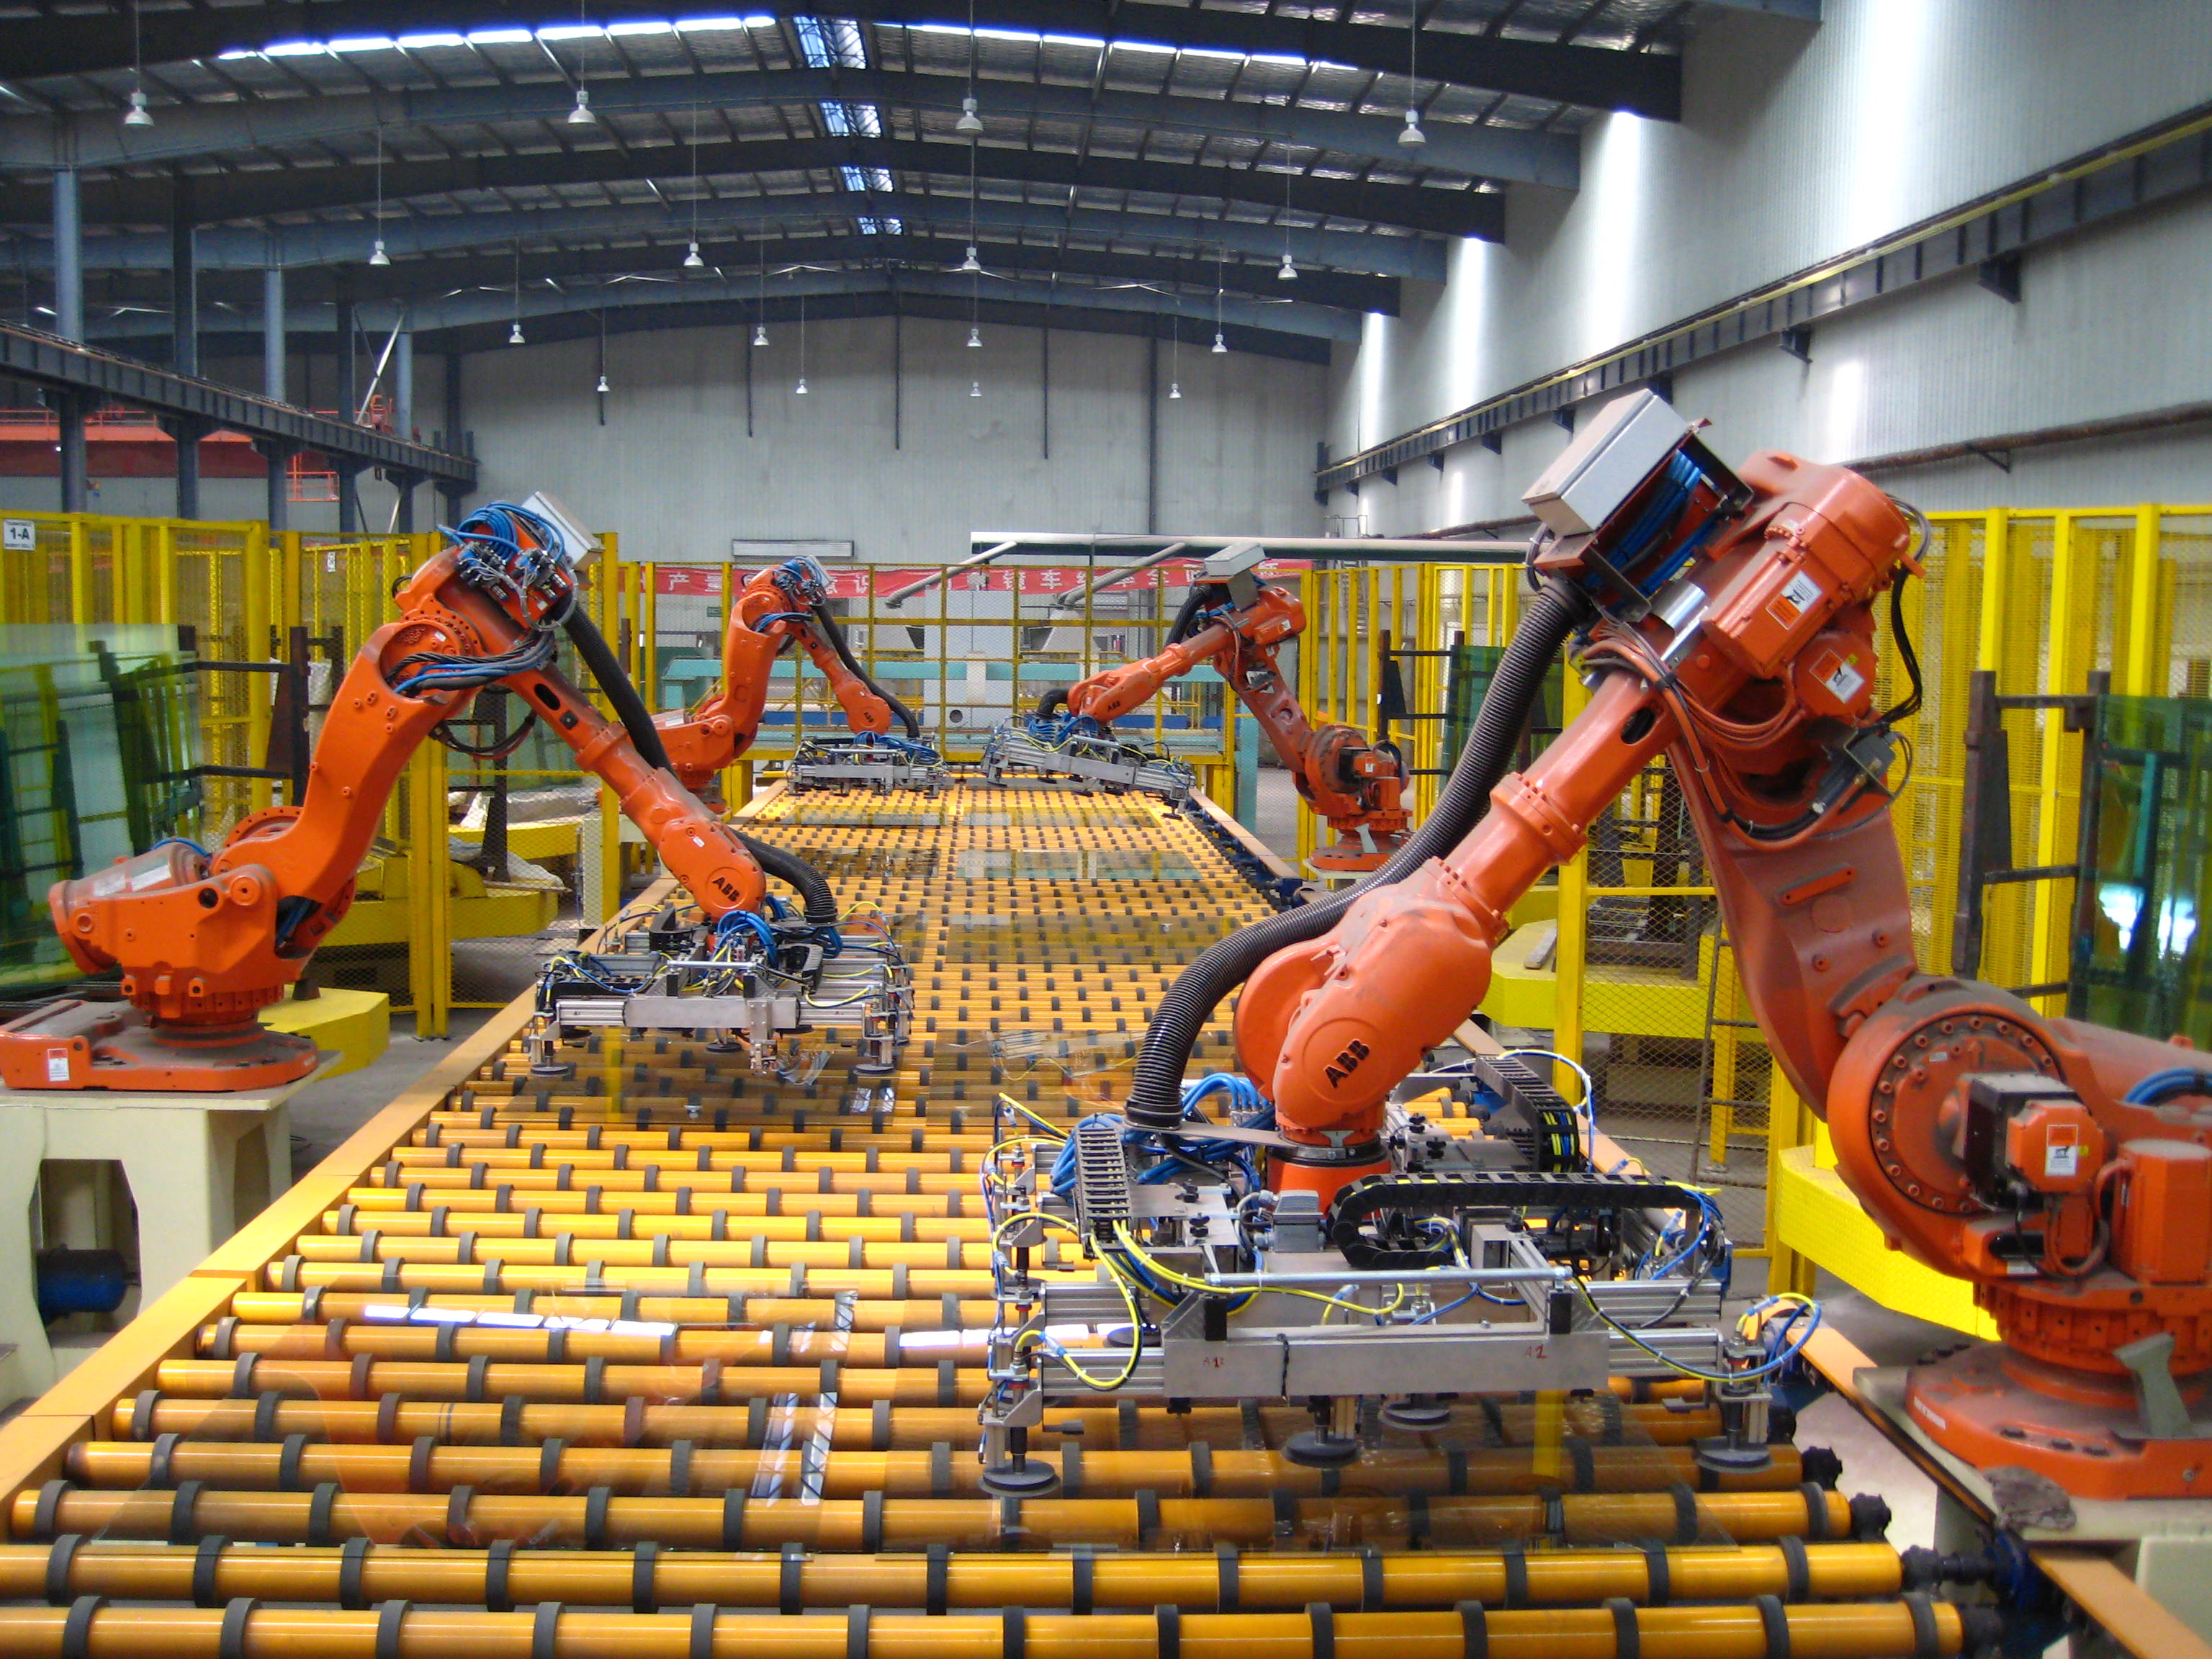
\includegraphics[width=8cm]{figs/industrial_robot.jpg}
    \end{center}
    \caption{Robots en líneas de ensamblaje}
    \label{fig:robIndustrialChain}
  \end{figure}\   

  \item \textit{Soldadura.} Es utilizada para realizar la unión de estructuras mecánicas debido a su alta precisión y capacidad de realizar 
                            la misma soldadura perfecta una y otra vez. Además, también son usados para soldar placas de circuitos.
  \begin{figure} [h!]
    \begin{center}
      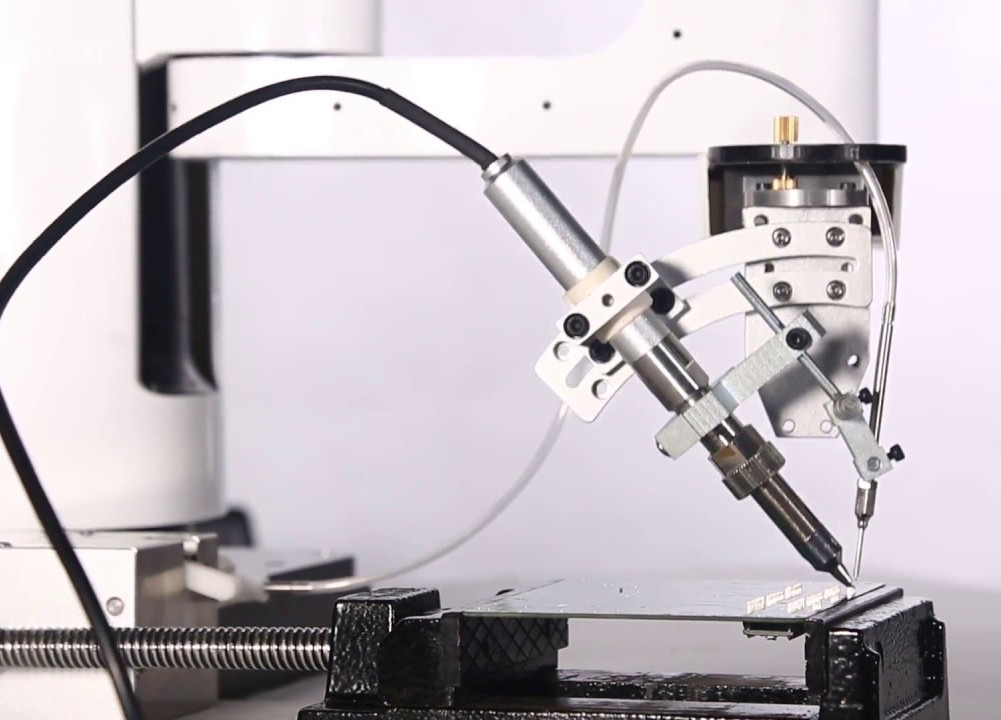
\includegraphics[width=8cm]{figs/solder_robot.jpg}
    \end{center}
    \caption{Robot Dobot M1 realizando una soldadura con estaño}
    \label{fig:robSoldering}
  \end{figure}\ 
\newpage
  \item \textit{Investigación y desarrollo en laboratorios.} Los brazos robóticos realizan tareas de laboratorio repetitivas y precisas, 
                              lo que puede acelerar el proceso de investigación y desarrollo de nuevos productos médicos. Uno de los usos más 
                              frecuentes es preparar y procesar muestras en investigaciones científicas. En concreto, pueden desempeñar tareas
                              como la extracción de \ac{ADN}, la separación de componentes, la adición de reactivos y el análisis de muestras 
                              químicas, entre otros. Esto ayuda a reducir los errores humanos y garantizar la integridad y reproducibilidad 
                              de los experimentos llevados a cabo.
  
  \begin{figure} [h!]
    \begin{center}
      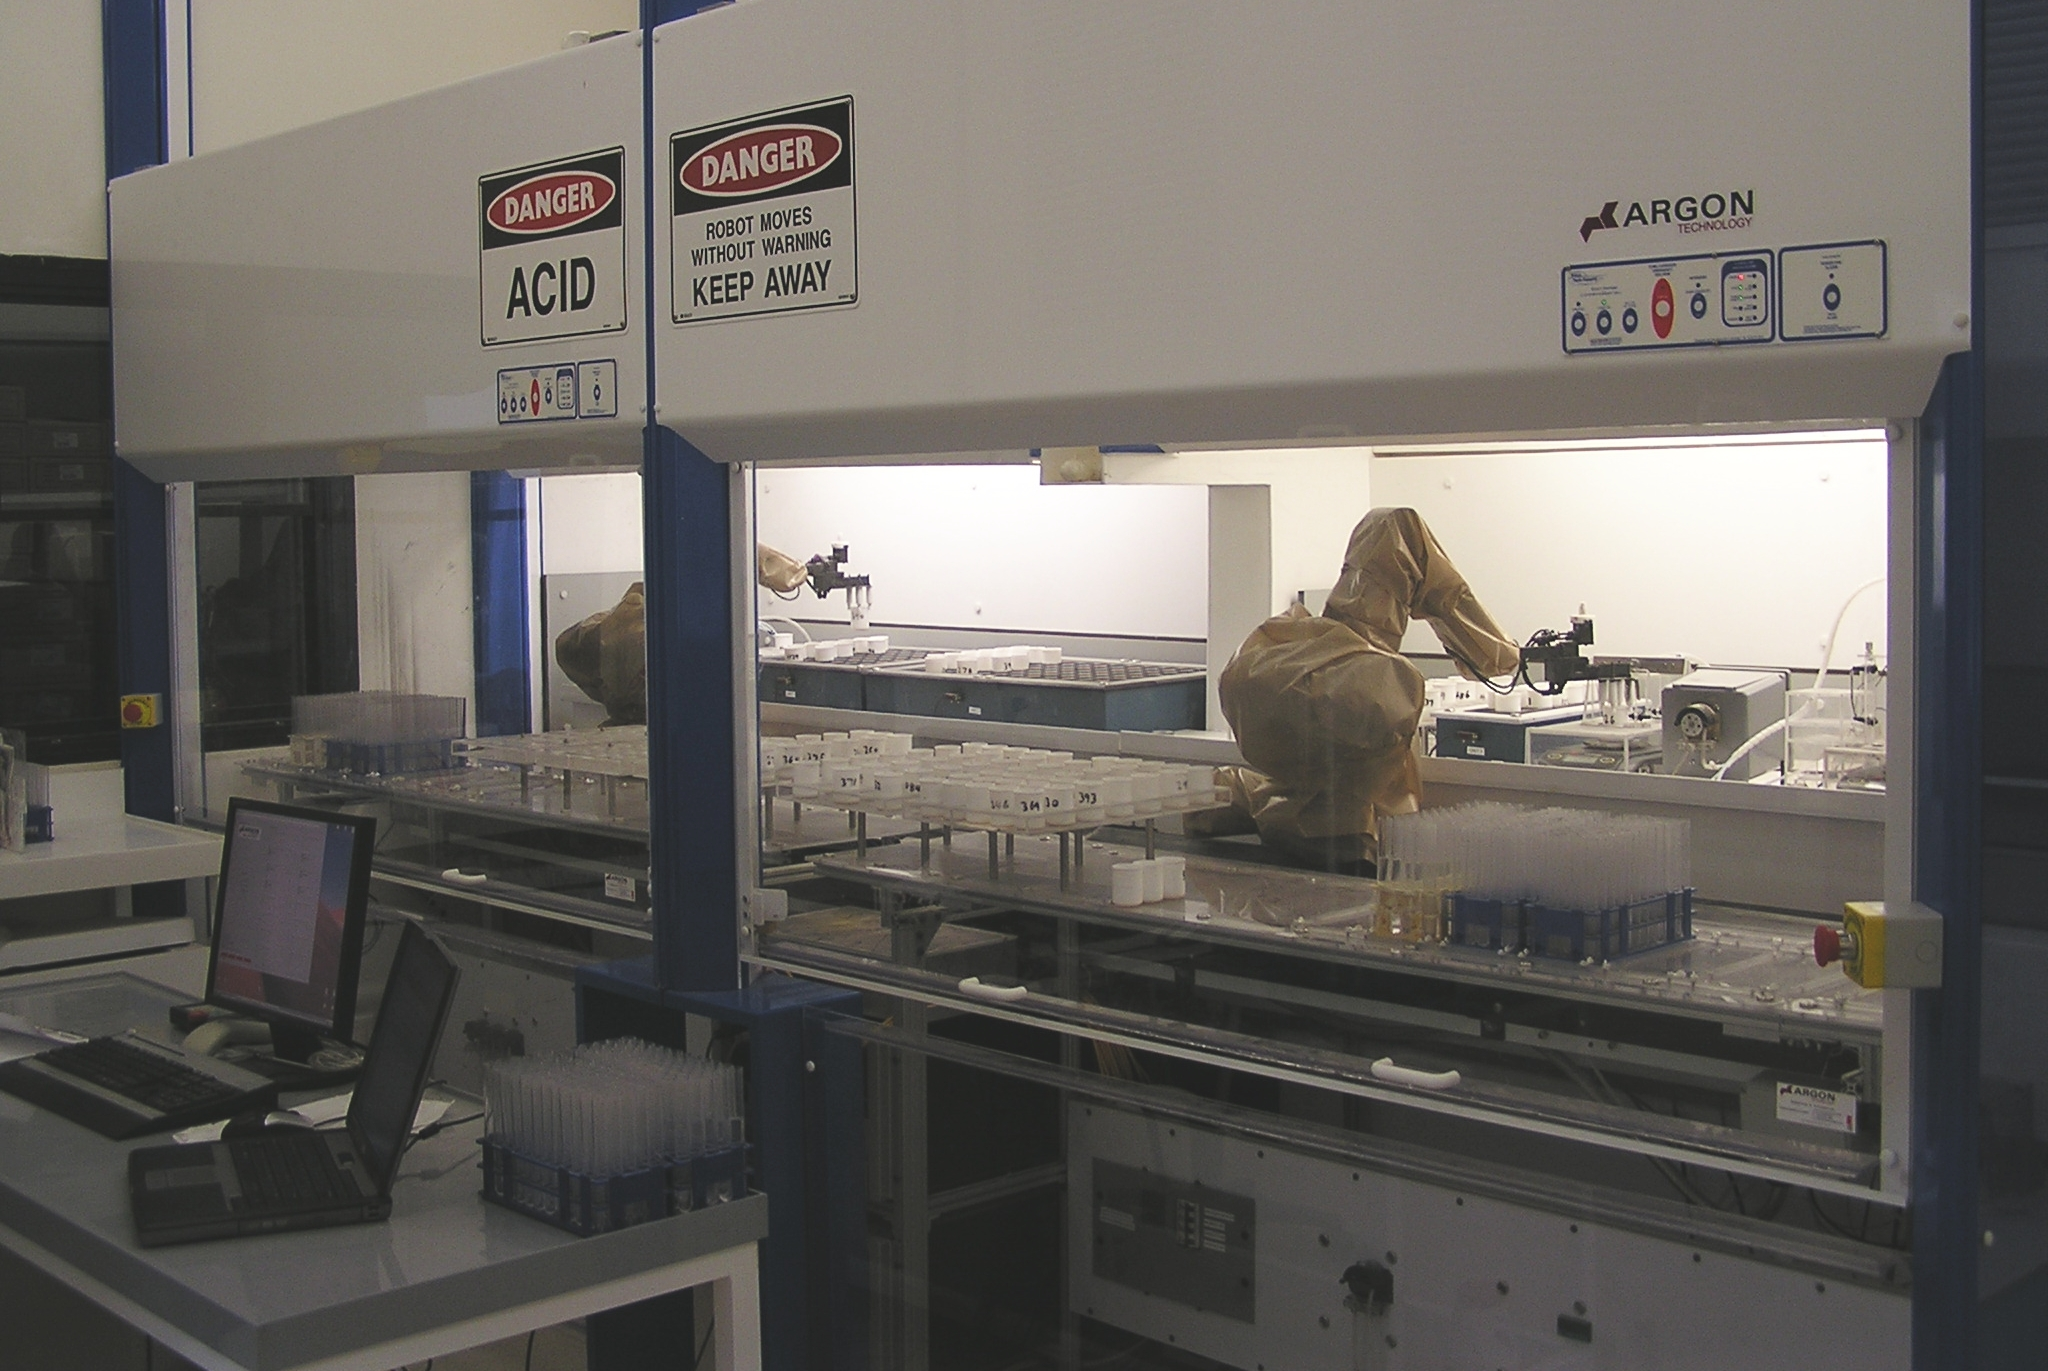
\includegraphics[width=8cm]{figs/lab_robot.jpg}
    \end{center}
    \caption{Robots en el ámbito científico}
    \label{fig:robLaboratory}
  \end{figure}\ 

 \end{itemize}\



\section{Robótica en educación}
\label{sec:segundaseccion}
La robótica en la educación es una disciplina que ha adquirido una gran relevancia en los últimos años debido a la creciente necesidad 
de formar a las nuevas generaciones en competencias tecnológicas.
\subsection{Robótica en colegios e institutos}
En las escuelas, se ha convertido en una herramienta pedagógica eficaz para desarrollar habilidades y conocimientos en áreas como la programación, 
la matemática, la electrónica y la resolución de problemas. Esto es conocido como \ac{STEM}. Los 
estudiantes aprenden a diseñar, construir y programar robots simples para llevar a cabo una tarea específica, lo que les ayuda a comprender  
los conceptos de ciencia y tecnología de una manera más práctica e interactiva.\\
\begin{figure} [h!]
  \begin{center}
    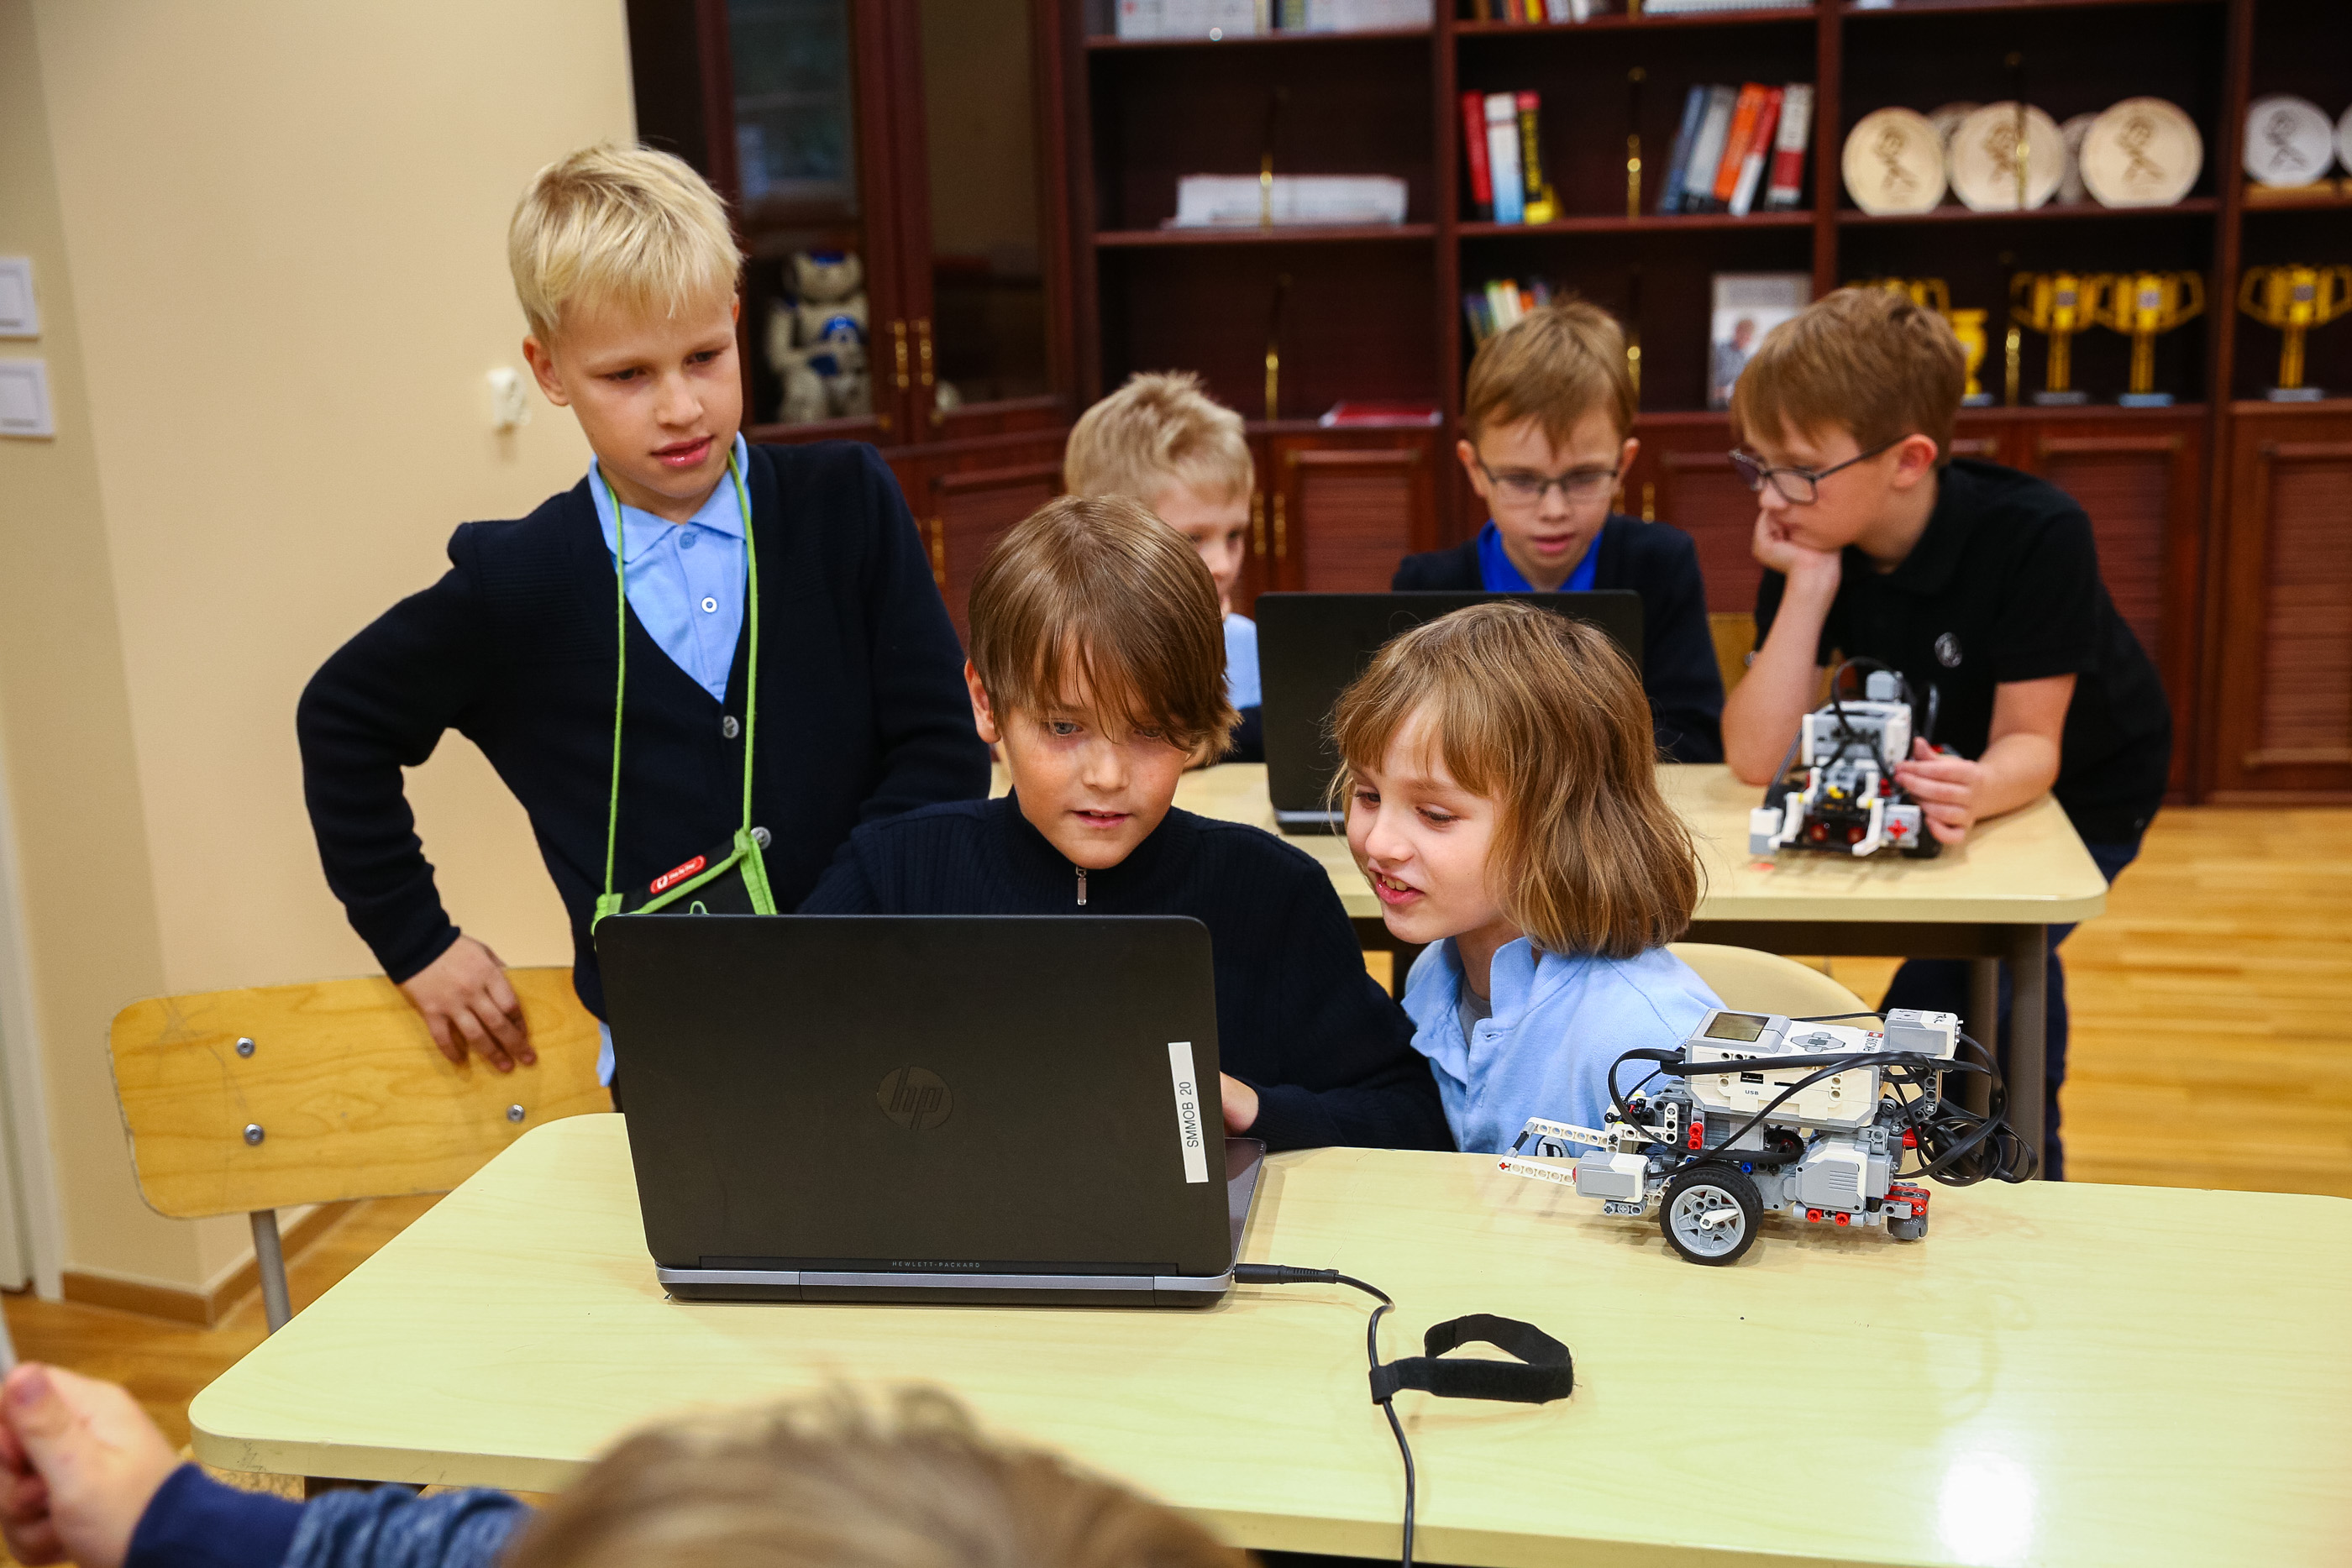
\includegraphics[width=8cm]{figs/education_robot.jpg}
  \end{center}
  \caption{Robots educativos Lego Mindstorms en escuelas.}
  \label{fig:robSecundaria}
\end{figure}\
\newpage
\subsection{Robótica en universidades}
En el nivel universitario, la robótica se ha convertido en una disciplina esencial para formar a los futuros ingenieros. Los estudiantes aprenden 
a diseñar y construir robots más avanzados, y refuerzan sus habilidades de programación y control de sistemas complejos. Además se hace uso de más tipos 
de robots, como pueden ser, industriales o plataformas robóticas móviles reales. Al ser sistemas usados en el mundo profesional, los estudiantes pueden 
aprender con el robot que usarán en un futuro. Aunque es verdad que las universidades disponen de algunas unidades, no siempre son accesibles para el 
estudiante por diversas razones.
\\\\
En resumen, la robótica en la educación es una herramienta poderosa para fomentar el aprendizaje y la innovación en las nuevas 
generaciones. Desde la escuela hasta la universidad, la robótica se ha convertido en una disciplina clave para formar a los futuros 
líderes tecnológicos del mundo.

\section{Robótica de bajo coste}
\label{sec:segundaseccion}
La robótica de bajo coste es un área de la robótica enfocada en el diseño y desarrollo de robots 
accesibles y asequibles. El objetivo principal de esta, es conseguir desarrollar tecnología robótica
barata, reduciendo la complejidad de los sistemas empleados y haciendo uso de materiales más económicos.

La disponibilidad de herramientas de fabricación de bajo costo, como la impresión 3D y el corte láser, 
han hecho posible que los usuarios puedan crear piezas y componentes robóticos personalizados a un 
precio más bajo que el de la fabricación tradicional.

La Ley de Moore es una ley teórica que establece que la capacidad de procesamiento de los microchips se duplica 
cada dos años. Esta observación, pese haberse dado hace casi 60 años, sigue siendo válida a día de hoy. Entre 
otras cosas, es lo que ha permitido el desarrollo de componentes electrónicos cada vez más pequeños, eficientes 
y potentes. La robótica de bajo coste es un claro ejemplo de cómo el crecimiento de la capacidad de computación y 
la disminución de los costes de producción ha llevado al abaratamiento de la robótica y de la electrónica en general.

Gracias a esto, la robótica de bajo coste, se basa en la filosofía `Hazlo tú mismo` o \ac{DIY}, que se enfoca en la creación de proyectos personalizados y 
asequibles utilizando tecnología de bajo costo y materiales comunes.

En resumen, la robótica de bajo costo es una consecuencia directa del crecimiento de la capacidad de computación, 
el abaratamiento de los precios de los componentes electrónicos y del enfoque \textit{DIY}. Estoque ha permitido la creación 
de robots avanzados y accesibles para el público general.
El desarollo de esta tecnología, permite que más personas puedan experimentar en este área de la ingeniería y desarrollar 
sus propias soluciones robóticas. 

\begin{figure} [h!]
  \begin{center}
    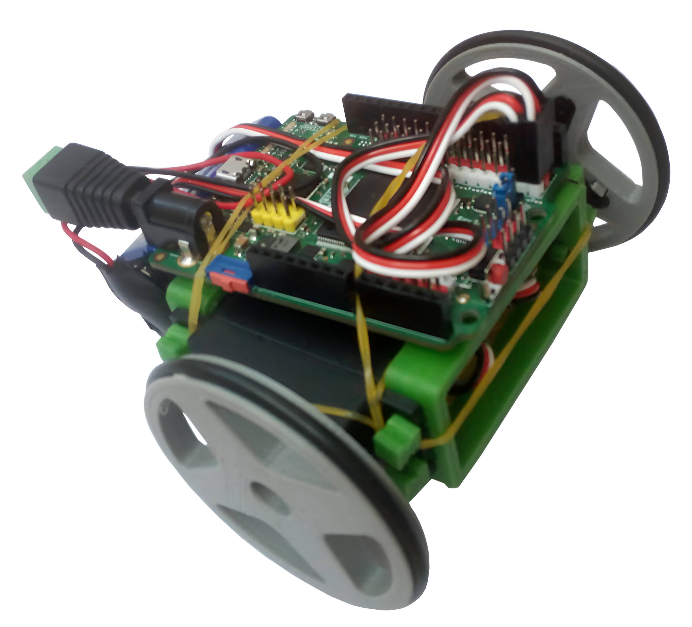
\includegraphics[width=8cm]{figs/icebot.png}
  \end{center}
  \caption{Robot IceBot que utiliza una FPGA libre Alhambra II.}
  \label{fig:robSecundaria}
\end{figure}\
\newpage

\paragraph{Referencias bibliográficas}
\label{sec:referencias}

Cita, sobre todo en este capítulo, referencias bibliográficas que respalden tu argumento. Para citarlas basta con poner la instrucción \verb|\cite| con el identificador de la cita. Por ejemplo: libros como \cite{vega12e}, artículos como \cite{vega19b}, URLs como \cite{vega19a}, tesis como \cite{vega18b}, congresos como \cite{vega18a}, u otros trabajos fin de grado como \cite{vega08b}.

Las referencias, con todo su contenido, están recogidas en el fichero \texttt{bibliografia.bib}. El contenido de estas referencias está en formato \texttt{BibTex}. Este formato se puede obtener en muchas ocasiones directamente, desde plataformas como \texttt{Google Scholar} u otros repositorios de recursos científicos.

Existen numerosos estilos para reflejar una referencia bibliográfica. El estilo establecido por defecto en este documento es APA, que es uno de los estilos más comunes, pero lo puedes modificar en el archivo \texttt{memoria.tex}; concretamente, cambiando el campo \verb|apalike| a otro en la instrucción \verb|\bibliographystyle{apalike}|. 

\

\

\

Y, para terminar este capítulo, resume brevemente qué vas a contar en los siguientes.
